\section{Shorter beams and the strip between them}
\label{beam:section}

The radial approximation theorem also permits a different coverage
strategy. Instead of enlarging two sweeps until they overlap, we shorten
them and cover their complement by horizontal cylinders. The shortening
saves area to first order, but the strip costs exactly that first-order
amount. A negative second-order term will make the total cost smaller.
We first realize the beams by the triangular construction of
Theorem~\ref{thm:radial}, then locate the complement and compute its cost.

\subsection{Euclidean coordinates and the cost normalization}\label{beam:geometry}

All notation in this section is local. We construct the cover for a
regular tetrahedron of edge length $2\sqrt{2}$; similarity then gives
the cover at every positive edge length, since both the covering cost
and $A_{\min}$ scale by the square of the similarity ratio.
Put $\beta=1/\sqrt{2}$ and write
\[
 P(x,y,t)=(\beta x,\beta y,t),\qquad
 K=\{P(x,y,t):-1\le t\le1,\ |x|\le1-t,\ |y|\le1+t\}.
\]
The map $P$ specifies physical Euclidean coordinates; $(x,y,t)$ are
parameters, so Euclidean lengths and areas must be computed after applying $P$.
The four vertices are $P(\pm2,0,-1)$ and $P(0,\pm2,1)$.
This is the image of the edge-four tetrahedron in
Section~\ref{sec:tetrahedron} under the Euclidean similarity
$(X,Y,Z)\mapsto(\beta X,\beta Y,-\beta Z)$.
Thus all six edges have length $2\sqrt2$, and \eqref{eq:min-area} gives
$A_{\min}(K)=\beta^2(4\sqrt2)=2\sqrt2$.
In the computations below we measure areas in units of
$\beta^2/\sqrt2$; this is a fixed cost normalization, distinct from
dividing each cylinder area by the projection in its own direction:
\begin{equation}\label{beam:normalization}
 A_{\min}(K)=2\sqrt{2},\qquad
 \text{normalized cost}=\frac{\text{perpendicular base area}}{\beta^2/\sqrt{2}}.
\end{equation}
The desired threshold in normalized cost is $4$.

We will repeatedly use the following exact conversion. For a compact planar
set $S\subset\mathbb R^2$ and $v\in\mathbb R^2$, the cylinder through $P(S,0)$ in
direction $(\beta v,1)$ has perpendicular base
$\pi_{(\beta v,1)^\perp}P(S,0)$. Its normalized cost is
\begin{equation}\label{beam:projection-factor}
 |S|\,g(v),\qquad
 g(v)=\frac{\sqrt{2}}{\sqrt{1+\beta^2|v|^2}}.
\end{equation}
Indeed, the horizontal area is $\beta^2|S|$, and orthogonal projection
multiplies it by the absolute inner product of the two unit plane normals,
namely $(1+\beta^2|v|^2)^{-1/2}$. Projection changes neither the cylinder nor
its direction. Normalizing that direction gives a unit axis as required.

\subsection{Compact beams and their finite coverings}

For $0<a<1/2$, define
\[
 R_a=2-a,\qquad r(p)=(p,1-p),\qquad
 v(p)=(1,-1)+aR_a(-p^2,(1-p)^2),\quad 0\le p\le1.
\]
With $c=(-1,-1)$, set
\begin{align*}
 H^-&=\{P(c+h r(p)+t v(p),t):0\le p\le1,\ 0\le h\le R_a,\ |t|\le1\},\\
 H^+&=\{P(-x,-y,t):P(x,y,t)\in H^-\}.
\end{align*}
The radial length $R_a=2-a$ shortens each central triangle by $a$.
Both beam regions are compact images of compact parameter sets.
At $t=0$ they are triangles on opposite corners of the square section
$[-1,1]^2$; Figure~\ref{beam:midsection} displays their central gap.
The regions $H^-$ and $H^+$ are the sets to be covered, whereas each
approximating cylinder will have one fixed direction.

\begin{figure}[htbp]
 \centering
 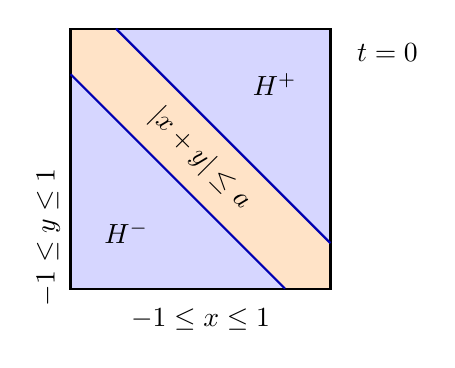
\begin{tikzpicture}[scale=1.65]
  \fill[blue!16] (-1,-1)--(.65,-1)--(-1,.65)--cycle;
  \fill[blue!16] (1,1)--(-.65,1)--(1,-.65)--cycle;
  \fill[orange!22] (-1,.65)--(.65,-1)--(1,-1)--(1,-.65)
                         --(-.65,1)--(-1,1)--cycle;
  \draw[thick] (-1,-1) rectangle (1,1);
  \draw[thick,blue!70!black] (-1,.65)--(.65,-1);
  \draw[thick,blue!70!black] (-.65,1)--(1,-.65);
  \node at (-.57,-.57) {$H^-$};
  \node at (.57,.57) {$H^+$};
  \node[fill=orange!22,inner sep=1.5pt,rotate=-45] at (0,0)
    {$|x+y|\le a$};
  \node[anchor=north] at (0,-1.08) {$-1\le x\le1$};
  \node[anchor=east,rotate=90] at (-1.17,0) {$-1\le y\le1$};
  \node[anchor=west] at (1.13,.82) {$t=0$};
 \end{tikzpicture}
 \caption{The beam sections at height zero, in parameter coordinates
 $(x,y)$, drawn with $a=0.35$. Their sloping sides satisfy
 $x+y=-a$ and $x+y=a$. The shaded closed band contains all points
 outside these two triangles. This value of $a$ illustrates the
 geometry only; the strict cost comparison will require smaller $a$.}
 \label{beam:midsection}
\end{figure}

\begin{lemma}\label{beam:finite-beams}
For fixed $a\in(0,1/2)$, partition $[0,1]$ into $k$ equal closed
intervals and choose a tag $p_I$ in each interval. The two beams admit
a covering by $2k$ cylinders with nondegenerate compact triangular
perpendicular bases, with axes parallel to $(\beta v(p_I),1)$ and
$(-\beta v(p_I),1)$, respectively. Their total normalized cost converges,
as $k\to\infty$, to
\begin{equation}\label{beam:C1}
 C_1=R_a^2\int_0^1 g(v(p))\,dp.
\end{equation}
In particular, for every $\eta>0$ a finite covering has cost at most
$C_1+\eta$.
\end{lemma}
\begin{proof}
We check the radial theorem in the physical horizontal plane, so its
area factor includes the scaling of both horizontal coordinates.
Take $e=(0,0,1)$, $p_0=(-\beta,-\beta,0)$ and
\[
 \mathbf a=(0,\beta,0),\qquad
 \mathbf b=(\beta,-\beta,0),\qquad
 \mathbf w(p)=(\beta v_1(p),\beta v_2(p),0).
\]
Then $\mathbf a+p\mathbf b=\beta(p,1-p,0)$ and
\[
 H^-=\{p_0+h(\mathbf a+p\mathbf b)+t(e+\mathbf w(p)):
       0\le p\le1,\ 0\le h\le R_a,\ |t|\le1\}.
\]
The hypotheses of Theorem~\ref{thm:radial} hold with constant cap $R_a$,
axial bound $1$ and
\[
 \mathbf w'(p)=-2aR_a(\mathbf a+p\mathbf b),\qquad
 |\det(\mathbf a,\mathbf b)|=\beta^2=\frac12,
 \qquad |\mathbf w(p)|^2=\beta^2|v(p)|^2.
\]
Consequently its one-beam limiting area is exactly
\begin{equation}\label{beam:physical-radial-cost}
 \frac{R_a^2}{4}\int_0^1\frac{dp}{\sqrt{1+\beta^2|v(p)|^2}}.
\end{equation}
For completeness, the explicit triangles in that theorem have
$A=2aR_a$, $B=aR_a$, $C=2(A+B)+1=6aR_a+1$. If $\delta=1/k$, their
individual perpendicular areas are
\[
 \frac{\delta\,[R_a+(A+C)\delta]^2}
      {4\sqrt{1+\beta^2|v(p_I)|^2}}.
\]
The orthogonal map $(X,Y,T)\mapsto(-X,-Y,T)$ gives the $k$ cylinders
for $H^+$ with the same areas. Adding the two costs and dividing by
$\beta^2/\sqrt2$ gives \eqref{beam:C1}.
\end{proof}

\subsection{The points left between the beams}

At $t=0$, the missed set is the diagonal band $|x+y|<a$ shown in
Figure~\ref{beam:midsection}. At other heights we enclose the missed
set in a tilted band with a uniform cubic error, using the transverse
coordinate $s$ and the coordinate $l$ along the diagonal:
\[
 s=x+y,\qquad l=(x-y)/2,\qquad f(t)=2at-2a^2t^3.
\]
For a constant $M>0$, to be chosen uniformly in the next lemma, define
\begin{align}
 W(t)&=\bigl(a(1-2t^2)
       +a^2t^2\{1+(1-|t|)^2+t^2\}+Ma^3\bigr)_+,
       \label{beam:width}\\
 G&=\{P(x,y,t)\in K:|s+f(t)l|\le W(t)\},\notag
\end{align}
where $q_+=\max(q,0)$.

\begin{lemma}\label{beam:coverage}
With $M=25$ in \eqref{beam:width}, one has
$K\subset H^-\cup H^+\cup G$ for every $0<a<1/2$.
\end{lemma}
\begin{proof}
Consider an interior point of $K$ outside both beams. Put
$U=x+1-t>0$ and $Y=y+1+t>0$. The strictly decreasing function
$U/p-Y/(1-p)$ runs from $+\infty$ to $-\infty$ on $(0,1)$, so there
is a $p$ satisfying
\[
 \frac Up-\frac Y{1-p}=-aR_a t,\qquad
 h=\frac Up+aR_a tp=\frac Y{1-p}-aR_a t(1-p).
\]
One of these expressions makes $h>0$ immediate, according to the sign of
$t$. They give exactly $P(x,y,t)=P(c+h r(p)+t v(p),t)$.
Because the point is outside $H^-$, necessarily $h>R_a$. Applying the same
argument to $(-x,-y,t)$ gives the corresponding reflected parameters,
also with radial parameter greater than $R_a$.

For the first representation put $d=h-R_a>0$, $q=2p-1$, and $b=R_a q/2$.
Direct substitution gives
\begin{equation}\label{beam:exact-gap}
 \begin{aligned}
 s&=-a-2atb+d,\\
 l&=t+b+dq/2-atQ,\qquad Q=R_a/4+b^2/R_a.
 \end{aligned}
\end{equation}
The reflected representation obeys these same identities with
$(-s,-l)$ in place of $(s,l)$. Since $|b|\le R_a/2<1$, the first identity
and its reflected version imply $|s|\le3a$, and then $0<d\le6a$.
Moreover $|l|\le1$ on $K$ and $Q\le R_a/2\le1$, so the second identity
gives the uniform estimate
\begin{equation}\label{beam:b-error}
 |b-(l-t)|\le4a.
\end{equation}
These bounds hold also for the reflected parameters. Since $R_a\ge3/2$
and $|l-t|\le2$, they give the numerical estimate
\begin{equation}\label{beam:uniform-constant}
 \left|Q-\frac{1+(l-t)^2}{2}\right|
 \le \frac a4+\frac{a b^2}{2R_a}
       +\frac{|b-(l-t)|\,|b+(l-t)|}{2}
 \le\left(\frac14+\frac13+6\right)a<10a.
\end{equation}
The bound is uniform, including for points tending to the boundary.

Combining the two equations in \eqref{beam:exact-gap} leaves a favorable
radial term:
\[
 s+2atl=-a+2at^2-2a^2t^2Q+d(1+atq)
 \ge -a+2at^2-a^2t^2\{1+(l-t)^2\}-20a^3,
\]
since $1+atq>0$. Reflection gives the complementary inequality
\[
 s+2atl\le a-2at^2+a^2t^2\{1+(l+t)^2\}+20a^3.
\]
Subtracting $2a^2t^3l$ from both inequalities cancels their mixed
quadratic terms, yielding
\begin{equation}\label{beam:central-strip}
 |s+f(t)l|\le a(1-2t^2)+a^2t^2(1+l^2+t^2)+20a^3.
\end{equation}
Finally the two coordinate bounds for $K$, applied to
$x=s/2+l$ and $y=s/2-l$, give
\[
 |l|\le1-|t|+|s|/2\le1-|t|+3a/2.
\]
Squaring shows $l^2\le(1-|t|)^2+3a+9a^2/4$.
Replacing $l^2$ by $(1-|t|)^2$ therefore adds at most
$(3+9a/4)a^3<5a^3$. Thus $M=25$ bounds the right side of
\eqref{beam:central-strip} by the expression inside the positive part in
\eqref{beam:width}. For such a point that expression is nonnegative,
so the point lies in $G$. We have proved coverage of the interior.
Both beams are compact, and $G$ is closed in the compact set $K$ because
$f$ and $W$ are continuous. Their finite union is closed and hence
contains the closure of the interior, namely all of $K$.
\end{proof}

\subsection{Finite horizontal cylinders for the strip}

The two beams now cover every point outside $G$. It remains to give
$G$ a finite covering whose cost can be combined with the beam cost.
\begin{lemma}\label{beam:finite-strip}
Fix $M$ as in Lemma~\ref{beam:coverage}. For every fixed $a\in(0,1/2)$
and $\eta>0$, the strip $G$ has a finite covering by cylinders with
compact rectangular perpendicular bases and normalized cost at most
$C_2+\eta$, where
\begin{equation}\label{beam:C2}
 C_2=2\sqrt{2}\int_{-1}^{1}
       \frac{W(t)}{\sqrt{1+(at-a^2t^3)^2}}\,dt.
\end{equation}
\end{lemma}
\begin{proof}
We construct the perpendicular rectangles explicitly. Define
$w(t)=(1+f(t)/2,1-f(t)/2)$, so that $s+f(t)l=w(t)\cdot(x,y)$.
Partition $[-1,1]$ into finitely many closed intervals $J$, choose
$t_J\in J$, and put
\[
 w_J=w(t_J),\quad n_J=(w_J/|w_J|,0),\quad
 A_J=\frac{\beta}{|w_J|}
 \left(\max_{t\in J}W(t)+3\max_{t\in J}|w(t)-w_J|\right).
\]
Choose a horizontal unit axis $u_J$ perpendicular to $n_J$. In its
perpendicular plane take the compact rectangle
\[
 B_J=\{z n_J+t(0,0,1): |z|\le A_J,\ t\in J\}.
\]
For a point of $G$ at height $t\in J$, its coordinate along $n_J$ is
$\beta w_J\cdot(x,y)/|w_J|$. Since $|(x,y)|\le3$ on $K$, its absolute
value is at most $A_J$. Thus $B_J+\mathbb R u_J$ covers that point.

The exact area of $B_J$ is $2A_J|J|$. Uniform continuity of $W$ and $w$
shows, as the mesh tends to zero, that the sum of these areas tends to
$\int_{-1}^{1}2\beta W(t)/|w(t)|\,dt$. Dividing by the cost unit in
\eqref{beam:normalization} and using
$|w(t)|=\sqrt{2}\sqrt{1+(at-a^2t^3)^2}$ gives
\eqref{beam:C2}. The freezing error tends to zero uniformly, including
at heights where $W$ vanishes. A sufficiently fine finite partition
therefore proves the asserted cost bound.
\end{proof}

\subsection{The strict saving survives finite approximation}\label{beam:cost-comparison}

\begin{proposition}[Cost of the shortened-beam construction]
\label{beam:counterexample}
For $a\in(0,1/2)$, fix $M=25$ in \eqref{beam:width} and put
$C(a)=C_1+C_2$, with $C_1,C_2$ as in
\eqref{beam:C1} and \eqref{beam:C2}.
For every $\zeta>0$, the tetrahedron $K$ has a finite cylinder cover
of normalized cost at most $C(a)+\zeta$, consisting of cylinders with
nondegenerate compact triangular perpendicular bases covering
$H^-\cup H^+$ and cylinders with horizontal axes and compact
rectangular perpendicular bases covering $G$.
Moreover,
\begin{equation}\label{beam:strict-gain}
 C(a)=4-\left(\frac{\sqrt2}{2}-\frac{19}{30}\right)a^2+O(a^3)
 \qquad(a\downarrow0).
\end{equation}
In particular, sufficiently small $a>0$ permits a finite cover whose
actual total base area is strictly below $A_{\min}(K)/2$.
\end{proposition}
\begin{proof}
For fixed $a$, choose the covers in Lemmas~\ref{beam:finite-beams}
and~\ref{beam:finite-strip} with excess costs at most $\zeta/2$ each.
Lemma~\ref{beam:coverage} shows that together they cover $K$, proving
the finite-cost bound. It remains to compute its limiting margin.

We now let $a\downarrow0$, keeping $M$ fixed. Write
$S_p=p^2+(1-p)^2$ and $T_p=p^4+(1-p)^4$. Uniformly in $p\in[0,1]$,
\begin{align*}
 g(v(p))
 &=\left(1-\frac{aR_a}{2}S_p+\frac{a^2R_a^2}{4}T_p\right)^{-1/2}\\
 &=1+\frac{aR_a}{4}S_p
      +a^2R_a^2\left(-\frac18T_p+\frac{3}{32}S_p^2\right)+O(a^3).
\end{align*}
The three needed integrals are
$\int_0^1S_p\,dp=2/3$, $\int_0^1T_p\,dp=2/5$, and
$\int_0^1S_p^2\,dp=7/15$. Hence
\begin{equation}\label{beam:C1-expansion}
 C_1=R_a^2+\frac{aR_a^3}{6}-\frac{a^2R_a^4}{160}+O(a^3)
     =4-\frac83a-\frac{11}{10}a^2+O(a^3).
\end{equation}
For $C_2$, its denominator is $1+O(a^2)$ and $W=O(a)$, so replacing
the denominator by $1$ changes the result by $O(a^3)$. Removing $Ma^3$
inside the positive part also has that error, because the positive-part
map is $1$-Lipschitz. Set $R=1/\sqrt{2}$. The leading expression
$a(1-2t^2)$ is positive exactly on $(-R,R)$. The quadratic perturbation
can change its sign only where $|1-2t^2|=O(a)$, a set of length $O(a)$
around the two simple zeros. On that set the integrand is $O(a^2)$.
It follows that
\begin{align}
 C_2
 &=4\sqrt{2}\int_0^R
     \left[a(1-2t^2)+a^2t^2\{1+(1-t)^2+t^2\}\right]dt+O(a^3)
       \notag\\
 &=\frac83a+\left(\frac{26}{15}-\frac{\sqrt{2}}2\right)a^2+O(a^3).
       \label{beam:C2-expansion}
\end{align}
Combining \eqref{beam:C1-expansion} and \eqref{beam:C2-expansion}
proves \eqref{beam:strict-gain}. The linear terms cancel, and the
quadratic coefficient is negative because $361/900<1/2$.
Hence $C(a)<4$ for all sufficiently small positive $a$.

To obtain a strict finite cover, first fix one such $a\in(0,1/2)$ and set
$\Delta=4-C_1-C_2>0$. Next choose the triangular beam covering of Lemma~\ref{beam:finite-beams}
and the rectangular strip covering, with excess costs each less than
$\Delta/3$. Together they cover $K$,
use unit axis directions and compact measurable perpendicular bases,
and have normalized cost less than $4$. By
\eqref{beam:normalization}, their actual total base area is less than
$4\beta^2/\sqrt{2}=\sqrt{2}=A_{\min}(K)/2$.
The parameter order is thus to fix $M=25$, then a sufficiently small
positive $a$, and finally the two finite partitions. The finite errors
use only a portion of the strict saving. The similarity described at
the start of the section transports this triangle-and-rectangle cover
to every regular tetrahedron of positive edge length.
\end{proof}
